\documentclass[11pt,letterpaper]{article}

\usepackage[T1]{fontenc}
\usepackage[utf8]{inputenc}
\usepackage{newtxtext,newtxmath}
\usepackage[margin=1in]{geometry}
\usepackage{microtype}
\usepackage{amsmath}
\usepackage{booktabs,tabularx,longtable,array}
\usepackage[table]{xcolor}
\usepackage{enumitem}
\usepackage{caption}
\usepackage{xspace}
\usepackage{tikz}
\usetikzlibrary{arrows.meta,positioning}
\usepackage{pgfplots}
\pgfplotsset{compat=1.17}
\usepackage[numbers,sort&compress]{natbib}
\usepackage[hidelinks]{hyperref}
\usepackage[nameinlink,capitalise]{cleveref}

% QRED's venue is indexed under its Chinese title; print the journal's English name instead
\DeclareUnicodeCharacter{7DB2}{}\DeclareUnicodeCharacter{969B}{Journal of Internet Technology}
\DeclareUnicodeCharacter{8DEF}{}\DeclareUnicodeCharacter{6280}{}\DeclareUnicodeCharacter{8853}{}
\DeclareUnicodeCharacter{5B78}{}\DeclareUnicodeCharacter{520A}{}

\definecolor{accent}{HTML}{1D4ED8}
\definecolor{muted}{HTML}{525252}
\hypersetup{colorlinks=true,linkcolor=accent,citecolor=accent,urlcolor=accent}
\setlist{itemsep=2pt,topsep=4pt}
\captionsetup{font=small,labelfont=bf}
\newcolumntype{L}[1]{>{\raggedright\arraybackslash}p{#1}}
\newcolumntype{Y}{>{\raggedright\arraybackslash}X}

% a short box naming the studies that use a technique
\newcommand{\usedby}[1]{\par\smallskip\noindent\colorbox{accent!7}{\parbox{\dimexpr\linewidth-2\fboxsep}{\small\textbf{Used in the 50:} #1}}\par\smallskip}
\newcommand{\E}{\mathbb{E}}

% counts generated by review/scripts/make_techniques.py (do not edit by hand)
% generated by review/scripts/make_techniques.py (do not edit by hand)
\newcommand{\tAnyAC}{8\xspace}
\newcommand{\tAnyBandit}{2\xspace}
\newcommand{\tAnyDQN}{6\xspace}
\newcommand{\tAnyIL}{3\xspace}
\newcommand{\tAnyMARL}{4\xspace}
\newcommand{\tAnyMO}{2\xspace}
\newcommand{\tAnyOff}{1\xspace}
\newcommand{\tAnyPG}{12\xspace}
\newcommand{\tAnyTab}{6\xspace}
\newcommand{\tDeep}{36\xspace}
\newcommand{\tDesign}{43\xspace}
\newcommand{\tHybrid}{15\xspace}
\newcommand{\tN}{50\xspace}
\newcommand{\tPrimAC}{5\xspace}
\newcommand{\tPrimBandit}{2\xspace}
\newcommand{\tPrimDQN}{3\xspace}
\newcommand{\tPrimIL}{2\xspace}
\newcommand{\tPrimMARL}{4\xspace}
\newcommand{\tPrimMO}{2\xspace}
\newcommand{\tPrimOff}{1\xspace}
\newcommand{\tPrimPG}{6\xspace}
\newcommand{\tPrimTab}{6\xspace}
\newcommand{\tTooling}{8\xspace}
\newcommand{\tUnspecified}{11\xspace}
\newcommand{\tvAnyAC}{8}
\newcommand{\tvAnyBandit}{2}
\newcommand{\tvAnyDQN}{6}
\newcommand{\tvAnyIL}{3}
\newcommand{\tvAnyMARL}{4}
\newcommand{\tvAnyMO}{2}
\newcommand{\tvAnyOff}{1}
\newcommand{\tvAnyPG}{12}
\newcommand{\tvAnyTab}{6}
\newcommand{\tvDeep}{36}
\newcommand{\tvDesign}{43}
\newcommand{\tvHybrid}{15}
\newcommand{\tvN}{50}
\newcommand{\tvPrimAC}{5}
\newcommand{\tvPrimBandit}{2}
\newcommand{\tvPrimDQN}{3}
\newcommand{\tvPrimIL}{2}
\newcommand{\tvPrimMARL}{4}
\newcommand{\tvPrimMO}{2}
\newcommand{\tvPrimOff}{1}
\newcommand{\tvPrimPG}{6}
\newcommand{\tvPrimTab}{6}
\newcommand{\tvTooling}{8}
\newcommand{\tvUnspecified}{11}


\title{\textbf{Reinforcement Learning Techniques in Congestion Control}\\[4pt]
\Large A Companion Guide to the \tN Most-Cited Studies}
\author{Gaurab Baral \and Nityashree Vangala}
\date{CS 6043: Networking\\[2pt] Fall 2026}

\begin{document}
\maketitle

\begin{abstract}
Our report on the \tN most-cited studies of reinforcement learning (RL) for congestion control names many learning methods (Q-learning, DQN, PPO, A3C, DDPG, TD3, IMPALA, imitation learning, offline RL, contextual bandits, multi-agent and multi-objective RL) without explaining them. This companion explains each one for a reader who knows networking but not RL. For every technique we give the idea, the update rule, the reason a congestion-control designer would pick it, and the studies among the \tN that use it, with the details those studies report. We close with the ideas that cut across algorithms: partial observability and recurrent policies, reward design, training curricula, hybrids with classic controllers, and verification of trained policies. A table at the end maps all \tN studies to their technique, action and reward.
\end{abstract}

\tableofcontents
\bigskip

% ======================================================================
\section{How to read this guide}
\label{sec:read}

The companion report ranks the studies and discusses their design, testing and deployment. Here we cover only the learning methods. \Cref{sec:basics} introduces the vocabulary every later section relies on. \Cref{sec:value,sec:pg,sec:ac} cover the three families that train most of the controllers: value-based methods, policy-gradient methods and off-policy actor-critics. \Cref{sec:il,sec:offline,sec:bandit} cover methods that learn from an expert, from logs, or from one-step feedback. \Cref{sec:marl,sec:mo} cover settings with several agents or several objectives. \Cref{sec:cross} collects techniques that are used with any algorithm, and \cref{sec:tools} covers the studies that analyze or run trained policies instead of training them. \Cref{sec:choose} compares the families, and \cref{app:table} lists every study.

\paragraph{Where the labels come from.} Each study's technique comes from our coding of its full text, abstract or our knowledge of the paper (the source of each is listed in the companion report). Of the \tN studies, \tDesign propose or train a controller. We assign each of them one primary family; \cref{fig:counts} shows the counts. For \tUnspecified studies the source we coded says only ``deep RL'' and does not name an algorithm, and \tTooling studies are frameworks or analyses that train no controller of their own. Several studies combine families. MVFST-RL, for example, is a framework whose agent is trained with IMPALA, and ACC is a multi-agent system whose agents are DQNs. We discuss such studies in every section that applies.

\begin{figure}[t]
\centering
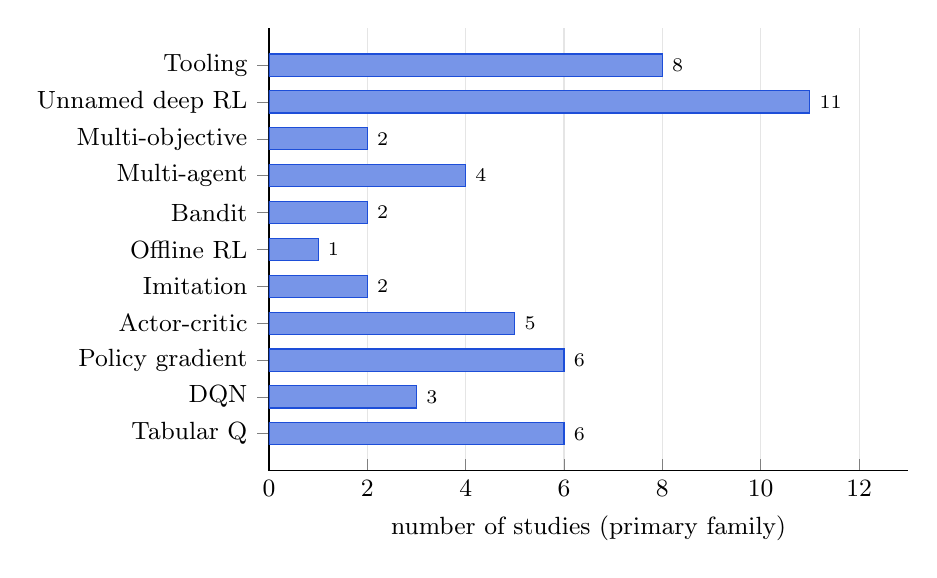
\begin{tikzpicture}
\begin{axis}[
  xbar, width=0.8\linewidth, height=7.2cm,
  xmin=0, xmax=13, bar width=8pt,
  symbolic y coords={Tooling,Unnamed deep RL,Multi-objective,Multi-agent,Bandit,Offline RL,Imitation,Actor-critic,Policy gradient,DQN,Tabular Q},
  ytick=data, y dir=reverse,
  xlabel={number of studies (primary family)},
  nodes near coords, nodes near coords align={horizontal},
  every node near coord/.append style={font=\scriptsize},
  tick label style={font=\small}, label style={font=\small},
  axis x line*=bottom, axis y line*=left, xmajorgrids, grid style={black!10},
]
\addplot[fill=accent!60, draw=accent] coordinates {
  (\tvPrimTab,Tabular Q) (\tvPrimDQN,DQN) (\tvPrimPG,Policy gradient) (\tvPrimAC,Actor-critic)
  (\tvPrimIL,Imitation) (\tvPrimOff,Offline RL) (\tvPrimBandit,Bandit) (\tvPrimMARL,Multi-agent)
  (\tvPrimMO,Multi-objective) (\tvUnspecified,Unnamed deep RL) (\tvTooling,Tooling)};
\end{axis}
\end{tikzpicture}
\caption{Primary technique family of the \tN studies. ``Unnamed deep RL'' (``Deep RL (n.s.)'' in \cref{app:table}) means the coded source does not name the algorithm. ``Tooling'' covers frameworks, verifiers and deployment methods.}
\label{fig:counts}
\end{figure}

% ======================================================================
\section{RL vocabulary in congestion-control terms}
\label{sec:basics}

\subsection{The Markov decision process}

RL models a controller as an \emph{agent} that interacts with an \emph{environment} in discrete steps~\cite{sutton2018reinforcement}. At step $t$ the agent observes a state $s_t$, picks an action $a_t$, receives a reward $r_t$, and the environment moves to $s_{t+1}$. A \emph{Markov decision process} (MDP) assumes that $s_{t+1}$ and $r_t$ depend only on $s_t$ and $a_t$, not on earlier history. In congestion control a step is usually one \emph{monitor interval}, about one round-trip time (RTT) long:

\begin{itemize}
  \item the \textbf{state} is a vector of recent statistics such as throughput, RTT, RTT gradient, loss rate and the current window;
  \item the \textbf{action} sets the congestion window (cwnd), the pacing rate, a video bitrate, a parameter of a classic algorithm, or, in a switch, a drop or ECN-marking decision;
  \item the \textbf{reward} scores the interval. Aurora's reward is $r_t = 10\cdot\text{throughput} - 1000\cdot\text{latency} - 2000\cdot\text{loss}$~\cite{jay2019aurora}.
\end{itemize}

\noindent The agent's behavior is a \emph{policy} $\pi$. A deterministic policy maps a state to an action, $a=\mu(s)$; a stochastic policy gives a probability for each action, $\pi(a\mid s)$. The goal is the policy that maximizes the expected \emph{discounted return}
\begin{equation}
G_t = \sum_{k=0}^{\infty} \gamma^k r_{t+k}, \qquad 0 \le \gamma < 1 .
\label{eq:return}
\end{equation}
The \emph{discount factor} $\gamma$ sets how far ahead the agent plans. With $\gamma=0.99$ and one step per RTT, rewards roughly 100 RTTs ahead still matter. This matters in congestion control, because filling a queue now raises delay for many later intervals.

\subsection{Value functions and the Bellman equation}

Most algorithms estimate how good a state or action is. The \emph{state value} $V^\pi(s)=\E_\pi[G_t\mid s_t=s]$ is the expected return from $s$ when following $\pi$. The \emph{action value} $Q^\pi(s,a)=\E_\pi[G_t\mid s_t=s,a_t=a]$ is the expected return after taking $a$ in $s$ and following $\pi$ afterwards. Their difference $A^\pi(s,a)=Q^\pi(s,a)-V^\pi(s)$ is the \emph{advantage}: how much better $a$ is than the policy's average action. The optimal action values satisfy the \emph{Bellman optimality equation}
\begin{equation}
Q^*(s,a) = \E\big[\, r + \gamma \max_{a'} Q^*(s',a') \,\big|\, s,a \big],
\label{eq:bellman}
\end{equation}
and acting greedily, $a=\arg\max_a Q^*(s,a)$, is optimal. Learning methods that bootstrap from \cref{eq:bellman} use the \emph{temporal-difference (TD) error} $\delta = r + \gamma \max_{a'} Q(s',a') - Q(s,a)$ as their learning signal.

\subsection{Distinctions that recur}

\paragraph{Discrete or continuous actions.} A discrete action space is a short menu, for example ``cwnd $-10$, $-1$, $0$, $+1$, $+10$''. Value-based methods need such a menu because they take a maximum over actions. A continuous action, such as a real-valued rate multiplier, needs a policy-gradient or actor-critic method. Of the coded design studies in \cref{app:table}, the early Q-learning and DQN controllers use discrete actions, while most PPO, DDPG and TD3 controllers use continuous ones.

\paragraph{On-policy or off-policy.} An \emph{on-policy} method (REINFORCE, A3C, PPO) learns only from data generated by its current policy and discards that data after each update. An \emph{off-policy} method (Q-learning, DQN, DDPG, TD3) can learn from data generated by any policy, including old versions of itself kept in a \emph{replay buffer}. Off-policy methods reuse data and are more sample-efficient, which matters when each sample is a real RTT of a real flow.

\paragraph{Exploration.} An agent must sometimes try actions it believes are worse, or it never learns that they are better. Value-based agents commonly use \emph{$\varepsilon$-greedy} exploration (a random action with probability $\varepsilon$). Stochastic policies explore by sampling. Deterministic actor-critics add noise to the action. On a live network, exploration has a cost, since a random action can overflow a buffer, which is why OnRL and Loki add safeguards (\cref{sec:online}).

\paragraph{Partial observability.} A sender sees only its own ACKs. It cannot see the bottleneck queue or the competing flows, so the true state is hidden and the problem is a \emph{partially observable} MDP (POMDP)~\cite{kaelbling1998planning}. \Cref{sec:pomdp} describes the two usual remedies: a history of observations in the state, or a recurrent network.

\paragraph{Function approximation.} With a handful of discretized states, $Q$ can be a table. With continuous measurements, the value function or policy is a parameterized function, usually a neural network with weights $\theta$. ``Deep RL'' means RL with neural-network approximators.

% ======================================================================
\section{Value-based methods}
\label{sec:value}

\subsection{Tabular Q-learning}

Q-learning~\cite{watkins1992q} keeps a table $Q(s,a)$ and, after each transition $(s,a,r,s')$, moves the entry toward the TD target:
\begin{equation}
Q(s,a) \leftarrow Q(s,a) + \alpha\big[\, r + \gamma \max_{a'} Q(s',a') - Q(s,a) \,\big],
\label{eq:qlearning}
\end{equation}
where $\alpha$ is a step size. Q-learning is off-policy, because the target uses the greedy action $\max_{a'}$ whatever action the agent actually took next. With enough exploration and a decaying step size, it converges to $Q^*$ in finite MDPs.

\paragraph{Why it fits congestion control.} The table is tiny, inference is a lookup, and the algorithm needs no neural-network library. These properties suit kernels, routers and constrained IoT devices. The cost is that the state must be discretized coarsely (for example, three RTT levels times three throughput levels), so the controller cannot react to fine differences, and each state must be visited often before its entries are reliable.

\subsection{Function approximation with coarse coding}

When the state is continuous, a table needs either coarse bins or a huge number of cells. Coarse coding represents a state by a set of overlapping binary features and stores a weight per feature, so that $Q(s,a)=\sum_i w_{i,a}\,\phi_i(s)$~\cite{sutton2018reinforcement}. Nearby states share features and therefore share what they learn. \emph{Tile coding} lays several offset grids (tilings) over the state space, and each active tile is a feature. \emph{Kanerva coding}~\cite{kanerva1988sparse} instead places prototype points in the state space and activates the prototypes close to the current state. Both keep memory fixed and updates linear, which is why they appear in resource-constrained designs.

\usedby{RL-TCP~\cite{kong2018improving} (tabular Q-learning over discretized TCP statistics, ns-2); QTCP~\cite{li2019qtcp} (Q-learning with generalized Kanerva coding, which adapts the prototype set during learning); SmartCC~\cite{li2019smartcc} (asynchronous Q-learning with hierarchical tile coding for multipath TCP); Li et al.~\cite{li2016learning} (Q-learning with function approximation to save memory on IoT devices); QRED~\cite{su2018qred} (Q-learning that tunes RED's maximum drop probability $\max_p$); G\'omez et al.~\cite{gomez2019intelligent} (Q-learning plus a neural congestion predictor for ECN-based AQM). TCP-RL's group-based RL for the initial window~\cite{nie2019tcprl} is closer to a bandit and is discussed in \cref{sec:bandit}.}

\subsection{Deep Q-Networks}

A Deep Q-Network (DQN)~\cite{mnih2015human} replaces the table with a neural network $Q_\theta(s,a)$ that takes the state and outputs one value per discrete action. Training minimizes the squared TD error
\begin{equation}
L(\theta) = \E_{(s,a,r,s')\sim\mathcal{D}}\Big[\big(r + \gamma \max_{a'} Q_{\theta^-}(s',a') - Q_\theta(s,a)\big)^2\Big].
\label{eq:dqn}
\end{equation}
Naively combining Q-learning with a neural network is unstable, and DQN adds two fixes. The \emph{replay buffer} $\mathcal{D}$ stores past transitions and samples mini-batches at random, which breaks the strong correlation between consecutive intervals of the same flow. The \emph{target network} $Q_{\theta^-}$ is a copy of the network that is updated only every few thousand steps, so the target does not move with every gradient step. \emph{Prioritized replay}~\cite{schaul2016prioritized} samples transitions with large TD error more often.

\paragraph{Why it fits congestion control.} DQN handles continuous, high-dimensional observations (for example, a long window of RTT samples) while keeping a discrete action menu that is easy to bound and to implement in a kernel. Inference is one forward pass followed by an $\arg\max$.

\usedby{TCP-Drinc~\cite{xiao2019drinc} (DQN whose network has convolutional and LSTM layers over a measurement history, ns-3); Owl~\cite{sacco2021owl} (DQN running in a Linux kernel module, with in-network signals added to end-to-end statistics); Kim et al.~\cite{kim2021deep} (DQN for AQM in fog and edge IoT networks); ACC~\cite{yan2021acc} (one DQN-style agent per switch that picks ECN marking thresholds, \cref{sec:marl}); DQL-MPTCP~\cite{pokhrel2021learning} (deep Q-learning combined with policy gradients and prioritized replay, \cref{sec:ac}); TCP-RL~\cite{nie2019tcprl} (deep RL that selects one of 14 congestion-control algorithms).}

% ======================================================================
\section{Policy-gradient methods}
\label{sec:pg}

\subsection{REINFORCE}

Policy-gradient methods parameterize the policy $\pi_\theta(a\mid s)$ directly and climb the gradient of the expected return $J(\theta)$. The policy-gradient theorem gives
\begin{equation}
\nabla_\theta J(\theta) = \E_{\pi_\theta}\big[\, \nabla_\theta \log \pi_\theta(a_t\mid s_t)\, \hat{A}_t \,\big],
\label{eq:pg}
\end{equation}
where $\hat{A}_t$ estimates how good $a_t$ was. REINFORCE~\cite{williams1992simple} uses the observed return $G_t$, often minus a baseline such as the average return. Actions that led to above-average returns become more likely. For a continuous action the policy is usually a Gaussian whose mean (and sometimes variance) the network outputs, so the action can be any real number, such as a rate multiplier. Plain REINFORCE has high variance and needs many episodes. Iroko~\cite{ruffy2018iroko} includes it as one of its baseline agents.

\subsection{Actor-critic and A3C}

An \emph{actor-critic} method learns two networks: the \emph{actor} $\pi_\theta$ and a \emph{critic} $V_\phi(s)$ that estimates state values. The critic supplies a lower-variance advantage, for example the one-step estimate $\hat{A}_t = r_t + \gamma V_\phi(s_{t+1}) - V_\phi(s_t)$ or the generalized advantage estimate (GAE)~\cite{schulman2016gae}, which averages multi-step estimates. The critic is trained by regression on returns.

A3C (asynchronous advantage actor-critic)~\cite{mnih2016a3c} runs many workers in parallel, each with its own copy of the environment. Workers compute gradients on their own experience and apply them asynchronously to shared parameters. Parallel workers decorrelate the data in the way a replay buffer does for DQN, and they shorten training wall time.

\usedby{QARC~\cite{huang2018qarc} (A3C chooses the video bitrate for real-time video, with a separate network that predicts video quality and feeds the agent); Fang et al.~\cite{fang2019rtc} (a PPO actor-critic for bandwidth estimation in real-time communication, below).}

\subsection{Proximal Policy Optimization (PPO)}

A large policy-gradient step can collapse a policy that took hours to train. PPO~\cite{schulman2017ppo} limits each update. It collects a batch of experience with the current policy $\pi_{\theta_\text{old}}$, forms the probability ratio $\rho_t(\theta)=\pi_\theta(a_t\mid s_t)/\pi_{\theta_\text{old}}(a_t\mid s_t)$, and maximizes the clipped objective
\begin{equation}
L^{\text{CLIP}}(\theta) = \E_t\Big[\min\big(\rho_t(\theta)\,\hat{A}_t,\ \operatorname{clip}(\rho_t(\theta),1-\epsilon,1+\epsilon)\,\hat{A}_t\big)\Big],
\label{eq:ppo}
\end{equation}
with $\epsilon$ around 0.2. Once the new policy moves an action's probability more than $\epsilon$ away from the old one, the objective stops rewarding further movement. PPO can then take several gradient steps on each batch without destabilizing. It is simple to implement, works with discrete and continuous actions, and is the default choice of many RL libraries, which partly explains its popularity in networking.

\paragraph{Aurora as the worked example.} Aurora~\cite{jay2019aurora} trains a PPO agent in a custom simulator. The state is a history of three scale-free statistics per monitor interval: the latency gradient, the latency ratio (current over minimum latency) and the sending ratio (packets sent over packets acknowledged). The action $a_t$ is a real number that changes the sending rate $x_t$:
\begin{equation}
x_t = \begin{cases} x_{t-1}\,(1+\alpha a_t) & a_t \ge 0,\\ x_{t-1}/(1-\alpha a_t) & a_t < 0,\end{cases}
\end{equation}
with a small scaling constant $\alpha$, so that equal positive and negative actions cancel. The reward is the weighted sum given in \cref{sec:basics}. Because the inputs are ratios, the same policy applies across link speeds, which helped it generalize to bandwidths far above its training range~\cite{jay2019aurora}.

\usedby{Aurora~\cite{jay2019aurora}; Genet~\cite{xia2022genet} (Aurora's formulation, trained with a curriculum, \cref{sec:curriculum}); MOCC~\cite{ma2022mocc} (PPO conditioned on objective weights, \cref{sec:mo}); Fang et al.~\cite{fang2019rtc} (PPO for real-time-communication bandwidth estimation, reporting a gap between simulated and real reward); BoB~\cite{bentaleb2022bob} (PPO warm-started with a heuristic, \cref{sec:hybrid}); Iroko~\cite{ruffy2018iroko} (PPO as one of three agents for data-center traffic control); Libra~\cite{du2025libra} (a policy-gradient agent whose proposed rate competes with a classic algorithm's, \cref{sec:hybrid}).}

\subsection{IMPALA and asynchronous training}

IMPALA~\cite{espeholt2018impala} separates \emph{actors}, which run the environment and record trajectories, from a central \emph{learner}, which updates the network. Actors keep running with slightly stale copies of the policy, so the data they send is off-policy with respect to the learner's current weights. IMPALA corrects for this lag with \emph{V-trace}, which weights each step's TD error by a truncated importance ratio $\min(\bar{c},\pi/\mu)$ between the learner policy $\pi$ and the actor policy $\mu$.

The separation matches a real network well. In a real stack the network does not pause while the agent computes, so an action decided now takes effect after a delay, and the sender keeps transmitting meanwhile. MVFST-RL~\cite{sivakumar2019mvfst} runs the policy asynchronously inside Facebook's QUIC implementation (mvfst) and trains it with IMPALA, treating the delay between observation and action as part of the problem.

\subsection{Policy gradients through a known reward}

When the reward is a known, differentiable function of the agent's output, the gradient can use that derivative instead of relying only on sampled returns. RL-CC~\cite{tessler2022rlcc} does this for data-center RDMA congestion control: its policy-gradient update uses the analytic derivative of the reward, and the problem is treated as multi-agent and partially observable, since each flow controls its own rate while sharing switches with the others. The reward is defined around the RTT inflation of each flow.

% ======================================================================
\section{Off-policy actor-critic methods}
\label{sec:ac}

\subsection{Deterministic policy gradient and DDPG}

For continuous actions a deterministic actor $\mu_\theta(s)$ can be trained by following the critic's gradient with respect to the action. The deterministic policy-gradient theorem~\cite{silver2014deterministic} gives
\begin{equation}
\nabla_\theta J \approx \E_{s\sim\mathcal{D}}\big[\, \nabla_a Q_\phi(s,a)\big|_{a=\mu_\theta(s)} \,\nabla_\theta \mu_\theta(s) \,\big].
\label{eq:dpg}
\end{equation}
In words, the critic tells the actor in which direction to nudge the action to increase value. DDPG~\cite{lillicrap2016ddpg} combines this with DQN's tricks: a replay buffer, slowly updated target networks for actor and critic, and exploration noise added to the action. The critic is trained on the TD target $r + \gamma Q_{\phi^-}(s', \mu_{\theta^-}(s'))$. Because DDPG is off-policy, it can learn from experience gathered by many distributed senders or by older policies.

\subsection{TD3}

DDPG's critic tends to overestimate values, and the actor then exploits those errors. TD3~\cite{fujimoto2018td3} adds three changes. It learns two critics and uses the smaller of their estimates in the target, $y = r + \gamma \min_{i=1,2} Q_{\phi_i^-}(s', \tilde{a}')$. It smooths that target by adding clipped noise to the target action, $\tilde{a}' = \mu_{\theta^-}(s') + \operatorname{clip}(\mathcal{N}(0,\sigma),-c,c)$. It updates the actor and the target networks less often than the critics, typically once every two critic steps.

\paragraph{Orca as the worked example.} Orca~\cite{abbasloo2020orca} keeps CUBIC running in the kernel on every ACK. Once per monitoring period, a TD3 agent in user space reads throughput, delay, loss and the current window and outputs $a\in[-1,1]$, and the window is set to
\begin{equation}
\text{cwnd} \leftarrow 2^{2a}\cdot \text{cwnd}_{\text{CUBIC}},
\end{equation}
so the agent can scale CUBIC's window by a factor between $1/4$ and $4$. Training uses many distributed actors in Mahimahi emulation that fill a shared replay buffer. The reward is based on \emph{power}, a ratio of throughput to delay. Off-policy learning lets Orca reuse every actor's experience, and the deterministic output is a single number that the kernel can apply cheaply.

\usedby{Orca~\cite{abbasloo2020orca} (TD3 with distributed actors); Abbasloo et al.'s DeepCC~\cite{abbasloo2021deepcc} (a DDPG plug-in that caps the window of an existing TCP scheme to meet a delay target on cellular links); DRL-CC~\cite{xu2019drlcc} (a deterministic policy-gradient actor-critic with an LSTM that sets the windows of all multipath TCP subflows); Naeem et al.~\cite{naeem2020software} (an actor-critic with a fuzzy normalized neural network, run centrally in an SDN controller for IoT multipath traffic); DQL-MPTCP~\cite{pokhrel2021learning} (deep Q-learning combined with policy gradients, LSTM and prioritized replay for multipath window and traffic split); Iroko~\cite{ruffy2018iroko} (DDPG as one of its agents).}

% ======================================================================
\section{Imitation learning}
\label{sec:il}

Imitation learning trains a policy to copy an \emph{expert} instead of maximizing a reward. In \emph{behavioral cloning} the expert labels states with actions and the policy is trained by ordinary supervised learning on those pairs. Cloning has a known weakness: the learned policy makes small mistakes, drifts into states the expert never visited, and has no labels for them. DAgger~\cite{ross2011dagger} fixes this by iterating. It runs the current learned policy, asks the expert what it would have done in each visited state, adds those labels to the dataset and retrains. The training data then covers the states the learner actually reaches.

The expert can be of two kinds in congestion control. An \emph{oracle} knows the simulated link's capacity and queue and can compute the ideal window, which is possible only in an emulator. An \emph{existing heuristic} such as BBR or CUBIC can be imitated anywhere, but the learner then inherits the heuristic's limits unless it is refined further with RL.

\usedby{Indigo, released with Pantheon~\cite{yan2018pantheon} (an LSTM policy trained to imitate an oracle that knows the ideal window of each emulated link, using DAgger-style iterations); Concerto~\cite{zhou2019concerto} (imitation learning on more than one million logged video-telephony sessions to coordinate the video codec with the transport rate); Eagle~\cite{emara2020eagle} (deep RL with an LSTM that uses BBR as an expert during training and then matches or beats it).}

% ======================================================================
\section{Offline RL}
\label{sec:offline}

Offline (or batch) RL learns a policy from a fixed dataset of transitions $\{(s,a,r,s')\}$ collected earlier by other policies, with no further interaction~\cite{levine2020offline}. It promises the benefit of RL without the risk of exploring on a live network. The difficulty is \emph{distribution shift}: an off-policy method such as DQN will happily assign high value to actions that never appear in the data, because nothing in the data contradicts its estimate, and the resulting policy then takes those untested actions. Offline RL algorithms therefore constrain the learned policy to stay near the actions in the dataset, or penalize value estimates for unseen actions, while still improving on the behavior that generated the data.

Unlike imitation learning, offline RL uses the reward. It can combine the best parts of several mediocre behaviors, so the learned policy can beat every policy in the dataset.

\usedby{Sage~\cite{yen2023sage}, which collects trajectories from a pool of existing heuristic controllers, learns a single policy from them offline, and in Internet and controlled tests outperforms the heuristics it observed. Concerto~\cite{zhou2019concerto} also learns only from logged sessions, but by imitation rather than reward maximization.}

% ======================================================================
\section{Bandits}
\label{sec:bandit}

A \emph{multi-armed bandit} is RL with a single step: the agent picks an arm (an action), receives a reward and the situation does not carry over to the next decision. The only difficulty is exploration, balancing arms that look good now against arms that have been tried too rarely. The \emph{upper confidence bound} (UCB) rule picks the arm with the highest optimistic estimate, its mean reward plus a bonus that shrinks as the arm is tried more often.

A \emph{contextual bandit} also observes a context vector $x$ before choosing. LinUCB~\cite{li2010contextual} assumes the expected reward of arm $k$ is linear in the context, $\E[r\mid x,k]=\theta_k^\top x$, keeps a ridge-regression estimate $\hat\theta_k = A_k^{-1} b_k$ for each arm, and picks
\begin{equation}
k^* = \arg\max_k \ \hat\theta_k^\top x + \alpha\sqrt{x^\top A_k^{-1} x},
\label{eq:linucb}
\end{equation}
where the second term is large when the context is unlike those seen for arm $k$. After the reward arrives, it updates $A_k \leftarrow A_k + x x^\top$ and $b_k \leftarrow b_k + r x$. Each step is a few small matrix operations, cheap enough to run online.

\paragraph{Why it fits congestion control.} Bandits suit decisions where the long-term effect of an action is small or can be ignored: which existing algorithm to use for the next period, or which initial window to give a new connection. Choosing among proven algorithms also keeps every action safe, since each arm is itself a deployed controller.

\usedby{Mutant~\cite{pappone2025mutant} (an online LinUCB bandit that switches among existing kernel congestion-control protocols in real time, rewarded by power); TCP-RL~\cite{nie2019tcprl} (group-based RL that picks the initial window for groups of users with similar network conditions, alongside deep RL that selects among 14 algorithms; it ran on a top global search engine's web servers for more than a year).}

% ======================================================================
\section{Multi-agent RL}
\label{sec:marl}

Congestion control is naturally multi-agent: every flow, or every switch, makes its own decision, and each decision changes the environment the others see. Multi-agent RL (MARL)~\cite{zhang2021multi} studies how several learners interact. Three designs are common.
\begin{itemize}
  \item \textbf{Independent learners.} Each agent treats the others as part of the environment. This is simple but non-stationary, because the other agents keep changing as they learn.
  \item \textbf{Parameter sharing.} All agents run copies of one policy and pool their experience. This suits homogeneous agents such as flows using the same protocol, or switches of the same type.
  \item \textbf{Centralized training with decentralized execution (CTDE).} During training, a critic sees global information (all flows' rates, the true queue); at run time each actor uses only local observations. MADDPG~\cite{lowe2017multi} is the best-known example.
\end{itemize}

\noindent The objective matters as much as the architecture. If each flow maximizes only its own reward, the learned policy tends to be greedy toward other copies of itself. Adding a fairness term or a shared reward makes the agents cooperate.

\usedby{Astraea~\cite{liao2024astraea} (several flows trained jointly in a faithful multi-flow environment, with local, global and historical observations and a reward that includes a fairness term; it reports near-optimal fairness and up to 8.4 times faster convergence); ACC~\cite{yan2021acc} (one agent per data-center switch adjusting ECN thresholds, trained offline and then online, deployed on production clusters of 300 machines); RL-CC~\cite{tessler2022rlcc} (multi-agent, partially observable RDMA congestion control); He et al.'s DeepCC~\cite{he2021deepcc} (one agent per multipath TCP subflow, with \emph{self-attention}~\cite{vaswani2017attention} so that each agent weighs the states of the other subflows).}

% ======================================================================
\section{Multi-objective and multi-task RL}
\label{sec:mo}

A scalar reward such as $10\cdot\text{thr} - 1000\cdot\text{lat} - 2000\cdot\text{loss}$ fixes one trade-off. A video call wants low delay, and a bulk backup wants throughput. Multi-objective RL~\cite{hayes2022practical} keeps a reward \emph{vector} $\mathbf{r}=(r_\text{thr}, r_\text{delay}, r_\text{loss})$ and a preference vector $\mathbf{w}$ that says how much each objective matters. The simplest approach, \emph{linear scalarization}, optimizes $\mathbf{w}^\top\mathbf{r}$. A \emph{preference-conditioned} policy $\pi(a\mid s,\mathbf{w})$ takes $\mathbf{w}$ as an extra input and is trained on many sampled preferences, so a single network covers the whole range of trade-offs and the application picks $\mathbf{w}$ at run time.

\usedby{MOCC~\cite{ma2022mocc} (a PPO policy with a preference sub-network that reads the objective weights; one model competes with the best specialized algorithm for each objective, and transfer learning lets it adapt to new objectives 14.2 times faster than prior work); AUTO~\cite{li2021auto} (multi-objective RL with a preference-adaptation model for satellite-ground networks).}

\paragraph{Multi-task learning.} A related idea trains one network on several tasks at once, so that shared layers learn features useful for all of them. Lei et al.~\cite{lei2020congestion} train a central agent in a software-defined network on congestion control with load balancing as an auxiliary task.

% ======================================================================
\section{Techniques that cut across algorithms}
\label{sec:cross}

\subsection{Handling partial observability: history and recurrence}
\label{sec:pomdp}

Because the sender cannot see the queue, a single interval's statistics do not identify the state. Two remedies appear. The first stacks the last $k$ observations into the state vector, as Aurora does with its history of latency gradients and ratios. The second uses a recurrent network, usually an LSTM~\cite{hochreiter1997long}, whose hidden state summarizes the history of observations it has seen. An LSTM can in principle remember longer patterns than a fixed window, at the cost of harder training. Convolutional layers over a history window are a third option, used by TCP-Drinc.

\usedby{LSTMs in Indigo~\cite{yan2018pantheon}, DRL-CC~\cite{xu2019drlcc}, TCP-Drinc~\cite{xiao2019drinc}, Eagle~\cite{emara2020eagle} and DQL-MPTCP~\cite{pokhrel2021learning}; observation histories in Aurora~\cite{jay2019aurora}, Genet~\cite{xia2022genet}, AUTO~\cite{li2021auto}, BoB~\cite{bentaleb2022bob} and Astraea~\cite{liao2024astraea}.}

\subsection{Reward design}
\label{sec:reward}

The reward is the controller's specification. The \tN studies use four kinds.
\begin{itemize}
  \item \textbf{Weighted sums} of throughput, delay and loss, as in Aurora, Genet and MOCC. The weights choose the operating point; a large delay weight produces a cautious controller.
  \item \textbf{Power}, throughput divided by delay, a classic measure of a good operating point used by Orca, Mutant and G\'omez et al.
  \item \textbf{Utility functions} that combine several terms into one score, used by Owl, DRL-CC and Libra.
  \item \textbf{Application metrics}, such as quality of experience (bitrate, stalls, frame delay) for real-time video in QARC, Fang et al., Loki, BoB and HRCC, or flow completion time for TCP-RL and Xie et al.
\end{itemize}
\noindent Fairness is rarely in the reward. Astraea and IEACC~\cite{yang2022ieacc} include it, and most other studies only measure it afterward.

\subsection{Training curricula}
\label{sec:curriculum}

\emph{Curriculum learning}~\cite{bengio2009curriculum} orders training data, usually from easy to hard. Genet~\cite{xia2022genet} applies this idea to network environments, with ``hard'' defined relative to rule-based baselines. It repeatedly searches the space of environment parameters (bandwidth, delay, queue size, loss) for settings where the current RL policy falls furthest behind a rule-based baseline, and adds those settings to training. Training then concentrates on the environments where the policy has the most to learn, rather than spreading effort over a uniform range where most environments are already solved. Genet's curriculum-trained policies beat both regularly trained RL policies and rule-based baselines, including in real environments.

\subsection{Online learning with safeguards}
\label{sec:online}

Training in a simulator and freezing the policy leaves a gap to the real network. The alternative is to keep learning in deployment, which requires limiting the damage exploration can do.

\usedby{OnRL~\cite{zhang2020onrl} (each user's device runs an agent that learns online in a mobile video service; the agents' experience is aggregated into one model, and a rule-based controller takes over when the learned policy behaves abnormally); Loki~\cite{zhang2021loki} (fuses a learned model with a reverse-engineered rule-based model through dual attention and trains online, evaluated in a commercial service over 101 million sessions); ACC~\cite{yan2021acc} (offline pre-training, then online training on the switches).}

\subsection{Hybrids: learning on top of classic control}
\label{sec:hybrid}

Of the \tDesign design studies, \tHybrid keep a classic algorithm or safeguard in the deployed control loop. These hybrids can use any RL algorithm. What they share is a division of labor: the classic algorithm reacts at ACK timescale with well-understood behavior, and the learned part adjusts it more slowly or chooses when to override it. The patterns differ in how much authority the learner has.

\begin{itemize}
  \item \textbf{Scale the classic output.} Orca's TD3 agent multiplies CUBIC's window (\cref{sec:ac}). Abbasloo et al.'s DeepCC caps the window of an existing scheme, and HRCC~\cite{wang2021hybrid} sets a gain on a heuristic bandwidth estimate.
  \item \textbf{Tune a parameter.} QRED tunes RED's drop probability, and ACC tunes ECN thresholds.
  \item \textbf{Select among algorithms.} TCP-RL and Mutant choose which existing algorithm runs.
  \item \textbf{Compete and commit.} Libra~\cite{du2025libra} lets a classic algorithm and an RL policy each propose a rate, tries both briefly and commits to the one with higher utility.
  \item \textbf{Split timescales.} Spine~\cite{tian2024spine} has a coarse DRL agent emit sub-policies that a lightweight executor applies at fine timescale, cutting control overhead by at least 80\%.
  \item \textbf{Warm-start or fall back.} BoB~\cite{bentaleb2022bob} warm-starts PPO with a heuristic, and OnRL falls back to rules when the policy misbehaves.
\end{itemize}

% ======================================================================
\section{Tooling: training platforms, verification and deployment}
\label{sec:tools}

\tTooling of the \tN studies train no controller of their own but shape how controllers are trained, checked or run.

\paragraph{Training platforms.} Pantheon~\cite{yan2018pantheon} provides emulators calibrated against real Internet paths and a common harness for comparing schemes. MVFST-RL~\cite{sivakumar2019mvfst} provides asynchronous IMPALA training inside a QUIC stack. OpenNetLab~\cite{eo2022opennetlab} combines a gym-style environment with distributed real nodes for real-time media. Iroko~\cite{ruffy2018iroko} emulates data-center topologies and compares PPO, REINFORCE and DDPG, and its authors report instability and overfitting to the training topology.

\paragraph{Formal verification.} A neural policy is a function that can be checked mathematically. DNN verifiers in the line of Reluplex~\cite{katz2017reluplex} encode a network with ReLU activations as constraints and ask a solver whether any input in a given range can produce a forbidden output, for example ``the rate increases even though loss is high''. Verily~\cite{kazak2019verily} applies such verifiers to deep-RL networking systems. Because an RL policy acts repeatedly, a property may only fail after several steps. whiRL~2.0~\cite{eliyahu2021whirl} therefore combines DNN verification with model checking over multiple steps, and it proves some requirements of trained policies, including Aurora's, while finding counterexamples for others.

\paragraph{Interpretation.} Metis~\cite{meng2020interpreting} explains deep-learning networking systems by converting a local policy into a decision tree (and a global, multi-component system into a hypergraph). A decision tree trained to mimic the network's outputs gives an operator readable rules and can be checked, debugged or even deployed in place of the network.

\paragraph{In-kernel inference.} LiteFlow~\cite{zhang2022liteflow} addresses where a trained network runs. It places a compact snapshot of the neural network on a kernel fast path for low-latency inference, and keeps a user-space slow path that tunes the model and updates the kernel snapshot. This avoids the round trip between kernel and user space that a user-space agent would otherwise pay on every decision.

% ======================================================================
\section{Comparing the families}
\label{sec:choose}

\Cref{tab:choose} summarizes when each family fits. Three trends show in the \tN studies. The early work (2016--2019) used tabular Q-learning and DQN with discrete window steps. From Aurora onward, continuous-action methods (PPO, DDPG, TD3) dominate the most-cited controllers. The newest designs lean on prior knowledge, through imitation of heuristics (Eagle), offline RL on heuristic logs (Sage), bandits over existing protocols (Mutant) or explicit hybrids (Orca, Libra, Spine).

\begin{table}[ht]
\centering
\small
\caption{Technique families in the \tN studies and the situations they fit.}
\label{tab:choose}
\begin{tabularx}{\linewidth}{@{}L{2.6cm}L{2.2cm}YL{3.1cm}@{}}
\toprule
Family & Actions & Fits when & Main risk \\
\midrule
Tabular Q-learning & discrete & state can be coarsely discretized; memory or code size is tight (kernel, IoT, router) & coarse states; slow learning \\
DQN & discrete & rich observations, small action menu & unstable training; overestimation \\
PPO / A3C & discrete or continuous & a simulator gives plentiful on-policy data & sample-hungry; sensitive to reward scale \\
DDPG / TD3 & continuous & data is costly and should be reused; many distributed actors & hyperparameter sensitivity; value overestimation (reduced by TD3) \\
IMPALA & either & acting and learning must run asynchronously, as in a real stack & stale-policy bias (corrected by V-trace) \\
Imitation learning & either & a good expert or oracle exists & cannot exceed the expert without further RL \\
Offline RL & either & logs of existing controllers are available; online exploration is unsafe & distribution shift to unseen actions \\
Contextual bandit & discrete & choosing among proven algorithms or settings; long-term effects small & ignores delayed consequences \\
Multi-agent RL & either & many flows or switches act together; fairness matters & non-stationarity; greedy equilibria \\
Multi-objective RL & either & applications need different trade-offs from one model & more training; preference coverage \\
\bottomrule
\end{tabularx}
\end{table}

% ======================================================================
\appendix
\section{Technique of each study}
\label{app:table}

Ranks follow the companion report. ``Family'' is the primary family used in \cref{fig:counts}; ``n.s.'' means the coded source does not name the algorithm, and ``n.r.'' that the reward is not reported there. Actions are marked continuous (cont.) or discrete (disc.) where we could code it. Rows coded from abstracts are lower bounds on what the papers contain.

{\small
\setlength{\tabcolsep}{3pt}
\begin{longtable}{@{}r L{3.0cm} L{1.9cm} L{4.6cm} L{2.2cm} L{2.0cm}@{}}
\toprule
\# & Study & Family & Technique & Action & Reward \\
\midrule
\endfirsthead
\toprule
\# & Study & Family & Technique & Action & Reward \\
\midrule
\endhead
\bottomrule
\endfoot
% generated by review/scripts/make_techniques.py (do not edit by hand)
1 & Aurora~\cite{jay2019aurora} & Policy gradient & PPO & rate (cont.) & throughput, delay, loss \\
2 & Orca~\cite{abbasloo2020orca} & Actor-critic & TD3 (distributed actors) & cwnd (cont.) & power \\
3 & Pantheon (Indigo)~\cite{yan2018pantheon} & Tooling & imitation learning from emulator oracles (Indigo, LSTM) & -- & -- \\
4 & QTCP~\cite{li2019qtcp} & Tabular Q & Q-learning + generalized Kanerva coding & cwnd (disc.) & throughput, delay \\
5 & Genet~\cite{xia2022genet} & Policy gradient & curriculum learning promoting environments where RL lags rule-based baselines & rate (cont.) & throughput, delay, loss \\
6 & TCP-RL~\cite{nie2019tcprl} & Bandit & group-based RL (IW) + deep RL (CCA selection among 14) & parameter; algorithm choice (disc.) & FCT, throughput \\
7 & DRL-CC (MPTCP)~\cite{xu2019drlcc} & Actor-critic & deterministic policy gradient actor-critic + LSTM & cwnd (cont.) & utility \\
8 & OnRL~\cite{zhang2020onrl} & Deep RL (n.s.) & online RL: per-user agents, aggregated model, safeguards against risky exploration & bitrate (cont.) & QoE \\
9 & Metis~\cite{meng2020interpreting} & Tooling & decision-tree and hypergraph interpretation of DL networking systems & -- & -- \\
10 & Owl~\cite{sacco2021owl} & DQN & DQN in a Linux kernel module & cwnd (disc.) & utility \\
11 & QARC~\cite{huang2018qarc} & Policy gradient & A3C + video-quality prediction network & bitrate (disc.) & QoE \\
12 & SmartCC~\cite{li2019smartcc} & Tabular Q & Q-learning + hierarchical tile coding (asynchronous) & cwnd (disc.) & throughput \\
13 & Sage~\cite{yen2023sage} & Offline RL & offline RL learning from a pool of existing heuristics' trajectories & cwnd (cont.) & throughput, delay \\
14 & Concerto~\cite{zhou2019concerto} & Imitation & custom imitation learning on $>$1M logged sessions & bitrate (cont.) & -- \\
15 & whiRL 2.0~\cite{eliyahu2021whirl} & Tooling & DNN verification + model checking of DRL policies & -- & -- \\
16 & Loki~\cite{zhang2021loki} & Deep RL (n.s.) & RL model fused with a reverse-engineered rule-based model (dual attention), trained online & bitrate (cont.) & QoE \\
17 & RL-TCP~\cite{kong2018improving} & Tabular Q & Q-learning & cwnd (disc.) & throughput, delay \\
18 & Verily~\cite{kazak2019verily} & Tooling & formal verification of DRL policies & -- & -- \\
19 & TCP-Drinc~\cite{xiao2019drinc} & DQN & DQN with CNN+LSTM & cwnd (disc.) & throughput, delay \\
20 & Eagle~\cite{emara2020eagle} & Imitation & DRL with LSTM guided by BBR as expert & rate & throughput, delay, loss \\
21 & DQL-MPTCP~\cite{pokhrel2021learning} & Actor-critic & deep Q-learning with policy gradients, LSTM, prioritized replay & cwnd; traffic split (cont.) & throughput, delay \\
22 & MOCC~\cite{ma2022mocc} & Multi-objective & PPO with preference sub-network + transfer learning (user- and kernel-space) & rate (cont.) & throughput, delay, loss \\
23 & DeepCC (Abbasloo et al.)~\cite{abbasloo2021deepcc} & Actor-critic & DDPG plug-in capping the cwnd of existing TCP & parameter (cont.) & delay \\
24 & DeepCC (He et al., MPTCP)~\cite{he2021deepcc} & Multi-agent & multi-agent DRL with self-attention & cwnd & throughput \\
25 & SDN actor-critic MPTCP for IoT~\cite{naeem2020software} & Actor-critic & actor-critic with fuzzy normalized NN & cwnd (cont.) & n.r. \\
26 & DRL initial window for 5G MEC~\cite{xie2019adaptive} & Deep RL (n.s.) & DRL (+supervised refinement) & parameter & FCT, loss \\
27 & RL BWE for RTC (Microsoft)~\cite{fang2019rtc} & Policy gradient & PPO (actor-critic) & bitrate (cont.) & QoE \\
28 & RL-CC (Tessler et al.)~\cite{tessler2022rlcc} & Multi-agent & policy gradient with analytic reward derivative (multi-agent, partially observable) & rate (cont.) & other \\
29 & Spine~\cite{tian2024spine} & Deep RL (n.s.) & hierarchical: light CC executor + coarse-grained DRL sub-policy generator & parameter (cont.) & n.r. \\
30 & Libra~\cite{du2025libra} & Policy gradient & classic and RL candidates compared in exploration/evaluation stages & rate (cont.) & utility \\
31 & DQN AQM for fog/edge IoT~\cite{kim2021deep} & DQN & DQN & drop/mark (disc.) & delay, throughput \\
32 & iCoCoA~\cite{donta2023icocoa} & Deep RL (n.s.) & DRL & parameter & n.r. \\
33 & Astraea~\cite{liao2024astraea} & Multi-agent & multi-agent DRL with a faithful multi-flow training environment & rate (cont.) & throughput, delay, loss, fairness \\
34 & MVFST-RL~\cite{sivakumar2019mvfst} & Tooling & IMPALA (asynchronous actor-learner, V-trace off-policy correction) with delayed actions & -- & throughput, delay \\
35 & AUTO~\cite{li2021auto} & Multi-objective & multi-objective RL + preference-adaptation model & rate (disc.) & throughput, delay \\
36 & Iroko~\cite{ruffy2018iroko} & Tooling & PPO; REINFORCE; DDPG & -- & utility, delay \\
37 & Multi-task DRL CC (SDN)~\cite{lei2020congestion} & Deep RL (n.s.) & multi-task DRL & rate & n.r. \\
38 & ACC~\cite{yan2021acc} & Multi-agent & multi-agent DRL per switch (offline + online training) & ECN threshold (disc.) & throughput, delay \\
39 & Q-learning TCP for memory-constrained IoT~\cite{li2016learning} & Tabular Q & Q-learning with function approximation & cwnd (disc.) & throughput, delay \\
40 & OpenNetLab~\cite{eo2022opennetlab} & Tooling & platform for training/evaluating RL RTC CC & -- & -- \\
41 & DRL age-of-information over TCP/IP~\cite{sert2018optimizing} & Deep RL (n.s.) & deep RL & rate & other \\
42 & BoB~\cite{bentaleb2022bob} & Policy gradient & PPO + heuristic warm start & bitrate (cont.) & QoE \\
43 & Mutant~\cite{pappone2025mutant} & Bandit & online contextual bandit (LinUCB) over a pool of existing protocols & algorithm choice (disc.) & power \\
44 & QRED~\cite{su2018qred} & Tabular Q & Q-learning tuning RED maxp & parameter (disc.) & other \\
45 & LiteFlow~\cite{zhang2022liteflow} & Tooling & kernel fast path for NN inference + userspace slow path for tuning & rate & -- \\
46 & HRCC~\cite{wang2021hybrid} & Deep RL (n.s.) & RL agent sets a gain on the heuristic (GCC-like) bandwidth estimate & parameter (cont.) & QoE \\
47 & Intelligent AQM with ECN~\cite{gomez2019intelligent} & Tabular Q & Q-learning (+ANN congestion predictor) & drop/mark (disc.) & power \\
48 & IEACC~\cite{yang2022ieacc} & Deep RL (n.s.) & DRL with edge-aided congestion degrees & rate & throughput, loss, fairness \\
49 & Hd-TCP~\cite{cui2020improving} & Deep RL (n.s.) & DRL & cwnd & throughput, delay \\
50 & AQM meets DRL~\cite{ma2021intelligent} & Deep RL (n.s.) & DRL & drop/mark & n.r. \\

\end{longtable}
}

\bibliographystyle{abbrvnat}
\bibliography{references,references_extra}

\end{document}
